\documentclass{article}

% Remember to also load the algostyle.sty file into your project.
\usepackage{algostyle}

% Insert new packages here.

\begin{document}
\begin{question}
Let $G = (V, E)$ be an undirected graph. A {\em $k$-orientation} assigns each edge a direction such that every vertex of $G$ has {\em at most} $k$ incoming edges. Describe an $O(m^2 \log n)$ algorithm to find the smallest $k$ for which $G$ has a $k$-orientation.

For example, the cube graph should return $2$, as shown below.

\begin{center}
    \begin{tikzpicture}
        \node[circle, very thick, draw] (a) {};
        \node[circle, very thick, draw, right = 2.5cm of a] (b) {};
        \node[circle, very thick, draw, below = 2.5cm of b] (c) {};
        \node[circle, very thick, draw, left = 2.5cm of c] (d) {};

        \node[circle, very thick, draw, above right = 1cm and 1cm of a] (e) {};
        \node[circle, very thick, draw, above right = 1cm and 1cm of b] (f) {};
        \node[circle, very thick, draw, above right = 1cm and 1cm of c] (g) {};
        \node[circle, very thick, draw, above right = 1cm and 1cm of d] (h) {};

        \draw[very thick] (a) -- (b) -- (c) -- (d) -- (a);
        \draw[very thick] (e) -- (f) -- (g) -- (h) -- (e);
        \draw[very thick] (a) -- (e);
        \draw[very thick] (b) -- (f);
        \draw[very thick] (c) -- (g);
        \draw[very thick] (d) -- (h);

        \node[circle, very thick, draw, right = 3.5cm of b] (i) {};
        \node[circle, very thick, draw, right = 2.5cm of i] (j) {};
        \node[circle, very thick, draw, below = 2.5cm of j] (k) {};
        \node[circle, very thick, draw, left = 2.5cm of k] (l) {};

        \node[circle, very thick, draw, above right = 1cm and 1cm of i] (m) {};
        \node[circle, very thick, draw, above right = 1cm and 1cm of j] (n) {};
        \node[circle, very thick, draw, above right = 1cm and 1cm of k] (o) {};
        \node[circle, very thick, draw, above right = 1cm and 1cm of l] (p) {};

        \draw[very thick, ->] (i) -- (j);
        \draw[very thick, ->] (j) -- (n);
        \draw[very thick, ->] (n) -- (m);
        \draw[very thick, ->] (m) -- (p);
        \draw[very thick, ->] (p) -- (l);
        \draw[very thick, ->] (l) -- (k);
        \draw[very thick, ->] (k) -- (j);
        \draw[very thick, ->] (i) -- (m);
        \draw[very thick, ->] (n) -- (o);
        \draw[very thick, ->] (o) -- (p);
        \draw[very thick, ->] (k) -- (o);
        \draw[very thick, ->] (l) -- (i);
    \end{tikzpicture}
\end{center}
\end{question}

\begin{solution}
    We can perform a binary search over possible values of $k$. 
    The maximum possible indegree of a vertex is the number of other vertices $n - 1$,
    therefore the binary search will have $O(\log n)$ iterations.
    For each $k$, we want to determine if a $k$-orientation is possible.

    For each edge $(v_i, v_j)$ on the original graph $G$, 
    represent it as a vertex $e_{i,j}$ in the flow network $F$,
    with directed edges of capacity 1 $(e_{i,j}, v_i)$ and $(e_{i,j}, v_j)$.
    Let every vertex $v_i$ have an edge of capacity $k$ pointing towards a supersink $t$,
    and let the supersource $s$ have an edge of capacity 1 pointing towards each edge-vertex $e_{i,j}$.

    \begin{center}


        \tikzset{every picture/.style={line width=0.75pt}} %set default line width to 0.75pt        

        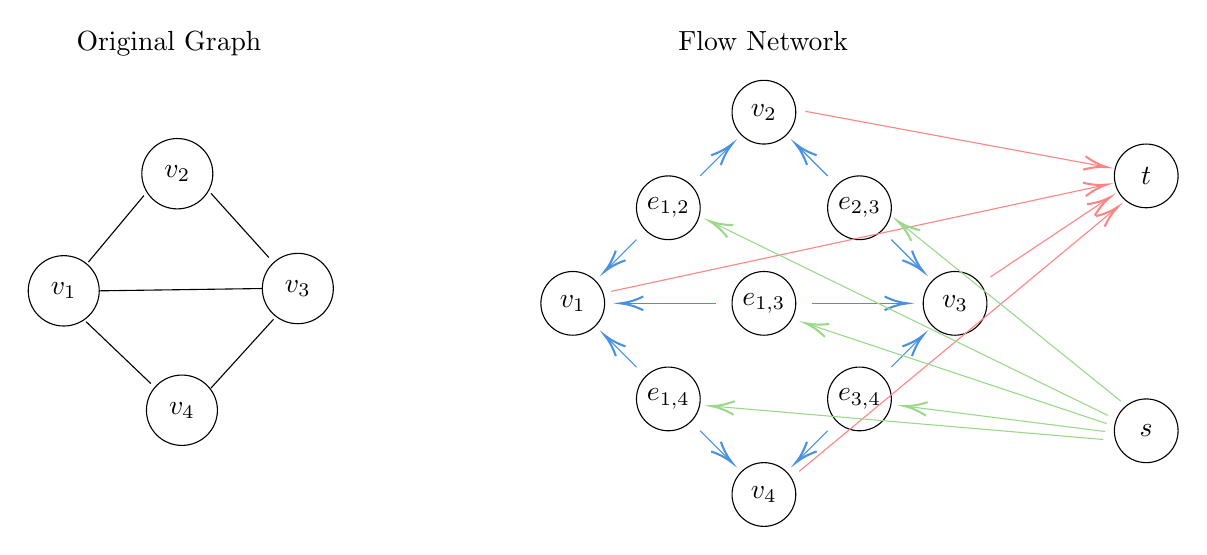
\begin{tikzpicture}[x=0.75pt,y=0.75pt,yscale=-1,xscale=1]
        %uncomment if require: \path (0,385); %set diagram left start at 0, and has height of 385
        
        %Shape: Ellipse [id:dp7189073146576883] 
        \draw   (311,212.55) .. controls (311,204.07) and (317.87,197.2) .. (326.35,197.2) .. controls (334.83,197.2) and (341.7,204.07) .. (341.7,212.55) .. controls (341.7,221.03) and (334.83,227.9) .. (326.35,227.9) .. controls (317.87,227.9) and (311,221.03) .. (311,212.55) -- cycle ;
        %Shape: Ellipse [id:dp7190373526868554] 
        \draw   (403.1,120.45) .. controls (403.1,111.97) and (409.97,105.1) .. (418.45,105.1) .. controls (426.93,105.1) and (433.8,111.97) .. (433.8,120.45) .. controls (433.8,128.93) and (426.93,135.8) .. (418.45,135.8) .. controls (409.97,135.8) and (403.1,128.93) .. (403.1,120.45) -- cycle ;
        %Shape: Ellipse [id:dp032192884290530355] 
        \draw   (495.2,212.55) .. controls (495.2,204.07) and (502.07,197.2) .. (510.55,197.2) .. controls (519.03,197.2) and (525.9,204.07) .. (525.9,212.55) .. controls (525.9,221.03) and (519.03,227.9) .. (510.55,227.9) .. controls (502.07,227.9) and (495.2,221.03) .. (495.2,212.55) -- cycle ;
        %Shape: Ellipse [id:dp20411891265090065] 
        \draw   (403.1,304.65) .. controls (403.1,296.17) and (409.97,289.3) .. (418.45,289.3) .. controls (426.93,289.3) and (433.8,296.17) .. (433.8,304.65) .. controls (433.8,313.13) and (426.93,320) .. (418.45,320) .. controls (409.97,320) and (403.1,313.13) .. (403.1,304.65) -- cycle ;
        %Shape: Ellipse [id:dp46522014420327773] 
        \draw   (357.05,166.5) .. controls (357.05,158.02) and (363.92,151.15) .. (372.4,151.15) .. controls (380.88,151.15) and (387.75,158.02) .. (387.75,166.5) .. controls (387.75,174.98) and (380.88,181.85) .. (372.4,181.85) .. controls (363.92,181.85) and (357.05,174.98) .. (357.05,166.5) -- cycle ;
        %Shape: Ellipse [id:dp36609483278040544] 
        \draw   (357.05,258.6) .. controls (357.05,250.12) and (363.92,243.25) .. (372.4,243.25) .. controls (380.88,243.25) and (387.75,250.12) .. (387.75,258.6) .. controls (387.75,267.08) and (380.88,273.95) .. (372.4,273.95) .. controls (363.92,273.95) and (357.05,267.08) .. (357.05,258.6) -- cycle ;
        %Shape: Ellipse [id:dp6169787510190654] 
        \draw   (449.15,258.6) .. controls (449.15,250.12) and (456.02,243.25) .. (464.5,243.25) .. controls (472.98,243.25) and (479.85,250.12) .. (479.85,258.6) .. controls (479.85,267.08) and (472.98,273.95) .. (464.5,273.95) .. controls (456.02,273.95) and (449.15,267.08) .. (449.15,258.6) -- cycle ;
        %Shape: Ellipse [id:dp17806484068164208] 
        \draw   (403.1,212.55) .. controls (403.1,204.07) and (409.97,197.2) .. (418.45,197.2) .. controls (426.93,197.2) and (433.8,204.07) .. (433.8,212.55) .. controls (433.8,221.03) and (426.93,227.9) .. (418.45,227.9) .. controls (409.97,227.9) and (403.1,221.03) .. (403.1,212.55) -- cycle ;
        %Shape: Ellipse [id:dp2742971363707991] 
        \draw   (449.15,166.5) .. controls (449.15,158.02) and (456.02,151.15) .. (464.5,151.15) .. controls (472.98,151.15) and (479.85,158.02) .. (479.85,166.5) .. controls (479.85,174.98) and (472.98,181.85) .. (464.5,181.85) .. controls (456.02,181.85) and (449.15,174.98) .. (449.15,166.5) -- cycle ;
        %Straight Lines [id:da5480851968233165] 
        \draw [color={rgb, 255:red, 74; green, 144; blue, 226 }  ,draw opacity=1 ]   (395.43,212.55) -- (351.38,212.55) ;
        \draw [shift={(349.38,212.55)}, rotate = 360] [color={rgb, 255:red, 74; green, 144; blue, 226 }  ,draw opacity=1 ][line width=0.75]    (10.93,-3.29) .. controls (6.95,-1.4) and (3.31,-0.3) .. (0,0) .. controls (3.31,0.3) and (6.95,1.4) .. (10.93,3.29)   ;
        %Straight Lines [id:da2311739831828017] 
        \draw [color={rgb, 255:red, 74; green, 144; blue, 226 }  ,draw opacity=1 ]   (441.48,212.55) -- (485.53,212.55) ;
        \draw [shift={(487.53,212.55)}, rotate = 180] [color={rgb, 255:red, 74; green, 144; blue, 226 }  ,draw opacity=1 ][line width=0.75]    (10.93,-3.29) .. controls (6.95,-1.4) and (3.31,-0.3) .. (0,0) .. controls (3.31,0.3) and (6.95,1.4) .. (10.93,3.29)   ;
        %Straight Lines [id:da5250177189758705] 
        \draw [color={rgb, 255:red, 74; green, 144; blue, 226 }  ,draw opacity=1 ]   (479.85,181.85) -- (493.79,195.79) ;
        \draw [shift={(495.2,197.2)}, rotate = 225] [color={rgb, 255:red, 74; green, 144; blue, 226 }  ,draw opacity=1 ][line width=0.75]    (10.93,-3.29) .. controls (6.95,-1.4) and (3.31,-0.3) .. (0,0) .. controls (3.31,0.3) and (6.95,1.4) .. (10.93,3.29)   ;
        %Straight Lines [id:da2789986925612953] 
        \draw [color={rgb, 255:red, 74; green, 144; blue, 226 }  ,draw opacity=1 ]   (387.75,273.95) -- (401.69,287.89) ;
        \draw [shift={(403.1,289.3)}, rotate = 225] [color={rgb, 255:red, 74; green, 144; blue, 226 }  ,draw opacity=1 ][line width=0.75]    (10.93,-3.29) .. controls (6.95,-1.4) and (3.31,-0.3) .. (0,0) .. controls (3.31,0.3) and (6.95,1.4) .. (10.93,3.29)   ;
        %Straight Lines [id:da7314310311366203] 
        \draw [color={rgb, 255:red, 74; green, 144; blue, 226 }  ,draw opacity=1 ]   (357.05,243.25) -- (343.11,229.31) ;
        \draw [shift={(341.7,227.9)}, rotate = 45] [color={rgb, 255:red, 74; green, 144; blue, 226 }  ,draw opacity=1 ][line width=0.75]    (10.93,-3.29) .. controls (6.95,-1.4) and (3.31,-0.3) .. (0,0) .. controls (3.31,0.3) and (6.95,1.4) .. (10.93,3.29)   ;
        %Straight Lines [id:da6944313456646956] 
        \draw [color={rgb, 255:red, 74; green, 144; blue, 226 }  ,draw opacity=1 ]   (357.05,181.85) -- (343.11,195.79) ;
        \draw [shift={(341.7,197.2)}, rotate = 315] [color={rgb, 255:red, 74; green, 144; blue, 226 }  ,draw opacity=1 ][line width=0.75]    (10.93,-3.29) .. controls (6.95,-1.4) and (3.31,-0.3) .. (0,0) .. controls (3.31,0.3) and (6.95,1.4) .. (10.93,3.29)   ;
        %Straight Lines [id:da2027359174386727] 
        \draw [color={rgb, 255:red, 74; green, 144; blue, 226 }  ,draw opacity=1 ]   (387.75,151.15) -- (401.69,137.21) ;
        \draw [shift={(403.1,135.8)}, rotate = 135] [color={rgb, 255:red, 74; green, 144; blue, 226 }  ,draw opacity=1 ][line width=0.75]    (10.93,-3.29) .. controls (6.95,-1.4) and (3.31,-0.3) .. (0,0) .. controls (3.31,0.3) and (6.95,1.4) .. (10.93,3.29)   ;
        %Straight Lines [id:da3616412388446115] 
        \draw [color={rgb, 255:red, 74; green, 144; blue, 226 }  ,draw opacity=1 ]   (449.15,151.15) -- (435.21,137.21) ;
        \draw [shift={(433.8,135.8)}, rotate = 45] [color={rgb, 255:red, 74; green, 144; blue, 226 }  ,draw opacity=1 ][line width=0.75]    (10.93,-3.29) .. controls (6.95,-1.4) and (3.31,-0.3) .. (0,0) .. controls (3.31,0.3) and (6.95,1.4) .. (10.93,3.29)   ;
        %Straight Lines [id:da9429301812307809] 
        \draw [color={rgb, 255:red, 74; green, 144; blue, 226 }  ,draw opacity=1 ]   (479.85,243.25) -- (493.79,229.31) ;
        \draw [shift={(495.2,227.9)}, rotate = 135] [color={rgb, 255:red, 74; green, 144; blue, 226 }  ,draw opacity=1 ][line width=0.75]    (10.93,-3.29) .. controls (6.95,-1.4) and (3.31,-0.3) .. (0,0) .. controls (3.31,0.3) and (6.95,1.4) .. (10.93,3.29)   ;
        %Straight Lines [id:da8040728505181638] 
        \draw [color={rgb, 255:red, 74; green, 144; blue, 226 }  ,draw opacity=1 ]   (449.15,273.95) -- (435.21,287.89) ;
        \draw [shift={(433.8,289.3)}, rotate = 315] [color={rgb, 255:red, 74; green, 144; blue, 226 }  ,draw opacity=1 ][line width=0.75]    (10.93,-3.29) .. controls (6.95,-1.4) and (3.31,-0.3) .. (0,0) .. controls (3.31,0.3) and (6.95,1.4) .. (10.93,3.29)   ;
        %Straight Lines [id:da0394296743645941] 
        \draw [color={rgb, 255:red, 255; green, 133; blue, 133 }  ,draw opacity=1 ]   (527.54,199.86) -- (583.44,162.6) ;
        \draw [shift={(585.1,161.49)}, rotate = 146.31] [color={rgb, 255:red, 255; green, 133; blue, 133 }  ,draw opacity=1 ][line width=0.75]    (10.93,-3.29) .. controls (6.95,-1.4) and (3.31,-0.3) .. (0,0) .. controls (3.31,0.3) and (6.95,1.4) .. (10.93,3.29)   ;
        %Shape: Ellipse [id:dp9833167211009697] 
        \draw   (587.3,151.15) .. controls (587.3,142.67) and (594.17,135.8) .. (602.65,135.8) .. controls (611.13,135.8) and (618,142.67) .. (618,151.15) .. controls (618,159.63) and (611.13,166.5) .. (602.65,166.5) .. controls (594.17,166.5) and (587.3,159.63) .. (587.3,151.15) -- cycle ;
        %Shape: Ellipse [id:dp3837851665480645] 
        \draw   (587.3,273.95) .. controls (587.3,265.47) and (594.17,258.6) .. (602.65,258.6) .. controls (611.13,258.6) and (618,265.47) .. (618,273.95) .. controls (618,282.43) and (611.13,289.3) .. (602.65,289.3) .. controls (594.17,289.3) and (587.3,282.43) .. (587.3,273.95) -- cycle ;
        %Straight Lines [id:da6831672600563432] 
        \draw [color={rgb, 255:red, 255; green, 133; blue, 133 }  ,draw opacity=1 ]   (438.51,120.04) -- (581.6,146.54) ;
        \draw [shift={(583.56,146.9)}, rotate = 190.49] [color={rgb, 255:red, 255; green, 133; blue, 133 }  ,draw opacity=1 ][line width=0.75]    (10.93,-3.29) .. controls (6.95,-1.4) and (3.31,-0.3) .. (0,0) .. controls (3.31,0.3) and (6.95,1.4) .. (10.93,3.29)   ;
        %Straight Lines [id:da6675479966913596] 
        \draw [color={rgb, 255:red, 255; green, 133; blue, 133 }  ,draw opacity=1 ]   (344.87,206.77) -- (581.61,155.77) ;
        \draw [shift={(583.56,155.35)}, rotate = 167.84] [color={rgb, 255:red, 255; green, 133; blue, 133 }  ,draw opacity=1 ][line width=0.75]    (10.93,-3.29) .. controls (6.95,-1.4) and (3.31,-0.3) .. (0,0) .. controls (3.31,0.3) and (6.95,1.4) .. (10.93,3.29)   ;
        %Straight Lines [id:da009389406098424535] 
        \draw [color={rgb, 255:red, 255; green, 133; blue, 133 }  ,draw opacity=1 ]   (435.44,293.5) -- (587.4,167.37) ;
        \draw [shift={(588.94,166.09)}, rotate = 140.31] [color={rgb, 255:red, 255; green, 133; blue, 133 }  ,draw opacity=1 ][line width=0.75]    (10.93,-3.29) .. controls (6.95,-1.4) and (3.31,-0.3) .. (0,0) .. controls (3.31,0.3) and (6.95,1.4) .. (10.93,3.29)   ;
        %Straight Lines [id:da5486511791559774] 
        \draw [color={rgb, 255:red, 156; green, 216; blue, 140 }  ,draw opacity=1 ]   (582.8,274.31) -- (488.08,262.28) ;
        \draw [shift={(486.09,262.03)}, rotate = 7.24] [color={rgb, 255:red, 156; green, 216; blue, 140 }  ,draw opacity=1 ][line width=0.75]    (10.93,-3.29) .. controls (6.95,-1.4) and (3.31,-0.3) .. (0,0) .. controls (3.31,0.3) and (6.95,1.4) .. (10.93,3.29)   ;
        %Straight Lines [id:da9163108855588193] 
        \draw [color={rgb, 255:red, 156; green, 216; blue, 140 }  ,draw opacity=1 ]   (583.56,270.47) -- (440.4,222.75) ;
        \draw [shift={(438.51,222.12)}, rotate = 18.43] [color={rgb, 255:red, 156; green, 216; blue, 140 }  ,draw opacity=1 ][line width=0.75]    (10.93,-3.29) .. controls (6.95,-1.4) and (3.31,-0.3) .. (0,0) .. controls (3.31,0.3) and (6.95,1.4) .. (10.93,3.29)   ;
        %Straight Lines [id:da2831037385459736] 
        \draw [color={rgb, 255:red, 156; green, 216; blue, 140 }  ,draw opacity=1 ]   (584.33,266.63) -- (394.25,173.88) ;
        \draw [shift={(392.46,173)}, rotate = 26.01] [color={rgb, 255:red, 156; green, 216; blue, 140 }  ,draw opacity=1 ][line width=0.75]    (10.93,-3.29) .. controls (6.95,-1.4) and (3.31,-0.3) .. (0,0) .. controls (3.31,0.3) and (6.95,1.4) .. (10.93,3.29)   ;
        %Straight Lines [id:da26760506964667985] 
        \draw [color={rgb, 255:red, 156; green, 216; blue, 140 }  ,draw opacity=1 ]   (590.47,259.73) -- (484.58,174.25) ;
        \draw [shift={(483.02,173)}, rotate = 38.91] [color={rgb, 255:red, 156; green, 216; blue, 140 }  ,draw opacity=1 ][line width=0.75]    (10.93,-3.29) .. controls (6.95,-1.4) and (3.31,-0.3) .. (0,0) .. controls (3.31,0.3) and (6.95,1.4) .. (10.93,3.29)   ;
        %Straight Lines [id:da280727472557901] 
        \draw [color={rgb, 255:red, 156; green, 216; blue, 140 }  ,draw opacity=1 ]   (582.03,278.15) -- (395.22,262.2) ;
        \draw [shift={(393.22,262.03)}, rotate = 4.88] [color={rgb, 255:red, 156; green, 216; blue, 140 }  ,draw opacity=1 ][line width=0.75]    (10.93,-3.29) .. controls (6.95,-1.4) and (3.31,-0.3) .. (0,0) .. controls (3.31,0.3) and (6.95,1.4) .. (10.93,3.29)   ;
        %Shape: Ellipse [id:dp6769620739170801] 
        \draw   (64,206.52) .. controls (64,197.16) and (71.66,189.57) .. (81.11,189.57) .. controls (90.56,189.57) and (98.21,197.16) .. (98.21,206.52) .. controls (98.21,215.88) and (90.56,223.47) .. (81.11,223.47) .. controls (71.66,223.47) and (64,215.88) .. (64,206.52) -- cycle ;
        %Shape: Ellipse [id:dp9713354816560407] 
        \draw   (118.72,150.09) .. controls (118.72,140.73) and (126.38,133.14) .. (135.83,133.14) .. controls (145.28,133.14) and (152.94,140.73) .. (152.94,150.09) .. controls (152.94,159.45) and (145.28,167.04) .. (135.83,167.04) .. controls (126.38,167.04) and (118.72,159.45) .. (118.72,150.09) -- cycle ;
        %Shape: Ellipse [id:dp7172794204591839] 
        \draw   (176.79,205.41) .. controls (176.79,196.05) and (184.44,188.46) .. (193.89,188.46) .. controls (203.34,188.46) and (211,196.05) .. (211,205.41) .. controls (211,214.78) and (203.34,222.36) .. (193.89,222.36) .. controls (184.44,222.36) and (176.79,214.78) .. (176.79,205.41) -- cycle ;
        %Shape: Ellipse [id:dp1551943312153521] 
        \draw   (120.95,264.05) .. controls (120.95,254.69) and (128.61,247.1) .. (138.06,247.1) .. controls (147.51,247.1) and (155.16,254.69) .. (155.16,264.05) .. controls (155.16,273.41) and (147.51,281) .. (138.06,281) .. controls (128.61,281) and (120.95,273.41) .. (120.95,264.05) -- cycle ;
        %Straight Lines [id:da7162073957205395] 
        \draw    (98.21,206.52) -- (176.79,205.41) ;
        %Straight Lines [id:da4380298493154313] 
        \draw    (119.72,160.64) -- (92.98,192.66) ;
        %Straight Lines [id:da8021206009212718] 
        \draw    (152.04,159.53) -- (179.91,190.45) ;
        %Straight Lines [id:da047926278130405064] 
        \draw    (123.07,251.19) -- (91.86,221.37) ;
        %Straight Lines [id:da09215970626535386] 
        \draw    (152.04,253.39) -- (182.13,220.27) ;
        
        % Text Node
        \draw (326.35,212.55) node    {$v_{1}$};
        % Text Node
        \draw (418.45,120.45) node    {$v_{2}$};
        % Text Node
        \draw (510.55,212.55) node    {$v_{3}$};
        % Text Node
        \draw (418.45,304.65) node    {$v_{4}$};
        % Text Node
        \draw (372.4,166.5) node    {$e_{1,2}$};
        % Text Node
        \draw (464.5,166.5) node    {$e_{2,3}$};
        % Text Node
        \draw (464.5,258.6) node    {$e_{3,4}$};
        % Text Node
        \draw (372.4,258.6) node    {$e_{1,4}$};
        % Text Node
        \draw (418.45,212.55) node    {$e_{1,3}$};
        % Text Node
        \draw (602.65,151.15) node    {$t$};
        % Text Node
        \draw (602.65,273.95) node    {$s$};
        % Text Node
        \draw (81.11,206.52) node    {$v_{1}$};
        % Text Node
        \draw (135.83,150.09) node    {$v_{2}$};
        % Text Node
        \draw (193.89,205.41) node    {$v_{3}$};
        % Text Node
        \draw (138.06,264.05) node    {$v_{4}$};
        % Text Node
        \draw (86,80) node [anchor=north west][inner sep=0.75pt]   [align=left] {Original Graph};
        % Text Node
        \draw (376,80) node [anchor=north west][inner sep=0.75pt]   [align=left] {Flow Network};
        
        
        \end{tikzpicture}
    \end{center}

    The direction that flow decides to take from each edge-vertex $e_{i,j}$ in the flow network represents 
    the orientation we provide to the edge in $G$. 
    Since all edges from the supersource have a weight of 1, each edge can only have one direction.
    Flow conservation states that the indegree of each vertex $v_i$ will be equal to 
    the total outflow towards $t$, therefore we ensure that the chosen directions form a $k$-orientation by 
    limiting the capacity of all edges $(v_i, t)$ to be equal to $k$.

    Use Dinic's Algorithm on this flow network, and check if the maximum flow is equal to 
    the number of edges in $G$. They are equal if and only if there exists a $k$-orientation for this $k$.

    The time complexity for this decision problem is $O(m|f|)$, but the maximum flow is limited by the number of edges, 
    so this is $O(m^2)$. Therefore the time complexity of the whole optimisation problem is $O(m^2 \log n)$.



\end{solution}
\end{document}